%!TEX root=../thesis.tex
\chapter{Technological stack} \label{cha:tech_stack}

There are a lot of technologies involved in this work. The whole system
architechture is composed of many different layers and the technological
stack under study is quite complex. Hence, this chapter aims at explaining
all its remarkable sections.


\section{FriWalk's architechture}\label{sec:friwalk_architechture}
The whole system architechture can be divided into two main parts. One that
is completely platform agnostic and another one that is platform dependent.
This distinction is due to the fact that different operating systems handle
3D graphics in many different ways, since the navigator application heavily
utilizes such primitives.
\begin{figure}[!htb]
    \center{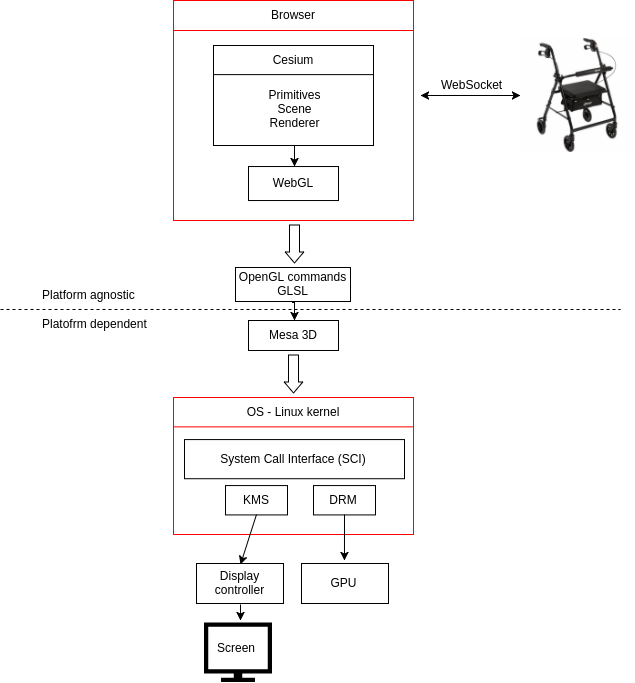
\includegraphics[width=0.6\linewidth]{system_architecture.png}}
    \caption{The FriWalk's system architecture.}
    \label{img:system_arch}
\end{figure}

As it is possible to see from Figure \ref{img:system_arch}, the first part includes
the walker assistant hardware, the browser running the
user interface (Google Chrome has been used in this study) and the component of
the OS which is responsible for implementing the OpenGL~\cite{woo1999opengl}
and the GLSL~\cite{marroquim2009introduction} libraries. On the other hand,
the platform dependent part includes the 3D graphics driver (eg. Mesa 3D for
Linux) and the OS kernel (eg. the Linux kernel). In the specific case of the
Linux kernel, it implements a System Call Interface (SCI) for interacting
with the Kernel Mode Setting (KMS)~\cite{linuxkms} and the Direct Rendering Manager
(DRM)~\cite{paul2000introduction}.


\subsection{Platform agnostic}
The 3D navigator application makes use of three pieces of information to move a
placeholder on the map: the \emph{latitude}, the \emph{longitude} and the
\emph{rotation}. These three values are not only the minimum amount of information
needed for the navigator to behave correctly, but also all the necessary.

From an high-level point of view, the walker assistant hardware can be regarded
as the portion of the system that is responsible for providing such data. Mooreover,
it can guarantee that data are available for the navigator at a fixed rate over
time using the WebSocket protocol~\cite{fette2011websocket}.
After receiving the data, the navigator properly moves the placeholder on the map.
This step can involves several operations, such as requesting a new tile for the
map, creating new 3D objects and so on. Consequently, the WebGL engine is responsible
for actually drawing the objects on the screen. A detailed description of how WebGL
behaves internally is given in Section \ref{sec:webgl}.

Finally, it is possible to say that the flow of information inside the platform
agnostic part of the system works as follows:
\begin{itemize}
    \item the FriWalk sends through a WebSocket the \emph{latitude}, the
        \emph{longitude} and the \emph{rotation} as a comma-separated string.
    \item the navigator running inside a browser receives the string, extracts
        the three values and uses them to build the objects needed to show the
        change on the screen.
    \item the framework powering the navigator actually performs the
        WebGL function calls.
    \item the graphical engine implemented inside the browser translates the WebGL
        function calls into generic OpenGL and GLSL commands, which are directly
        feeded to the graphical driver.
    \item the graphical hardware takes care of showing the scene on the screen.
\end{itemize}


\subsection{Platform dependent} \label{sec:platform_dependent}
This part of the system architechture highly depends on the operating system
running on the machine under test. In this work, a Linux-based OS (ie.
Ubuntu\footnote{\url{https://www.ubuntu.com}.})
has been used. Therefore the description may not fit, fully or partially, to
other operating systems like Apple Mac OS X, Microsoft Windows or other Linux
distributions.

The implementation of the OpenGL standard, the Mesa 3D Graphics Library. 
Graphics device drivers are implemented using two components: a User-Mode Driver
(UMD) and a Kernel-Mode Driver (KMD). The first can be seen as the interface
that can be used by other programs, while the second one directly interacts
with the KMS to set the display settings and with the DRM kernel subsystem
interfacing with the GPU(s). Starting from the 4.2 version of the Linux kernel,
multiple graphics drivers (eg. Mesa and AMD Catalyst) can share the same kernel
mode driver.


\section{Linux 3D graphics stack}
First it has to be underlined that this thesis refers only to the 3D part of the
graphics stack. This means that the window manager needs to ask the X11 server
only for the handle to a portion of the screen (i.e. the window).
3D graphics primitives do not need to interact any more with the X11 server. This
is needed to bypass the client-server architecture of X11 which is not suitable for
real-time 3D graphics and rendering, since it would have introduced more layers
of communication, delays and a high level of unpredictability.
This architecture is called
Direct Rendering Infrastructure (DRI)~\cite{paul2000introduction} and it is
necessary to overcome the scenario where only the X server is allowed to access
the graphics hardware. Moreover, DRI is composed by a user-space and a kernel-space
(ie. the DRM) part. This provides the building blocks that allow userspace applications
to directly access the graphics hardware in an efficient and safe way.
In addition, the DRM is a key component for the navigator application to achieve
hardware-accelerated 3D rendering and to manage video memory in Mesa.

As briefly described in Section \ref{sec:platform_dependent}, the Linux graphics
stack is quite complex and consists of many different layers in different parts
of the OS. The main ones are: the Mesa 3D Graphics Library, the System Call
Interface, the Kernel Mode Setting and the Direct Memory Manager.
As it is possible to see from Figure \ref{img:linux_graphics_stack}, the DRM and 
the display server belongs to the windowing system (eg. X11 or Wayland~\cite{wayland}) 
and it is not strictly necessary for applications directly using OpenGL function
calls.
\begin{figure}[!htb]
    \center{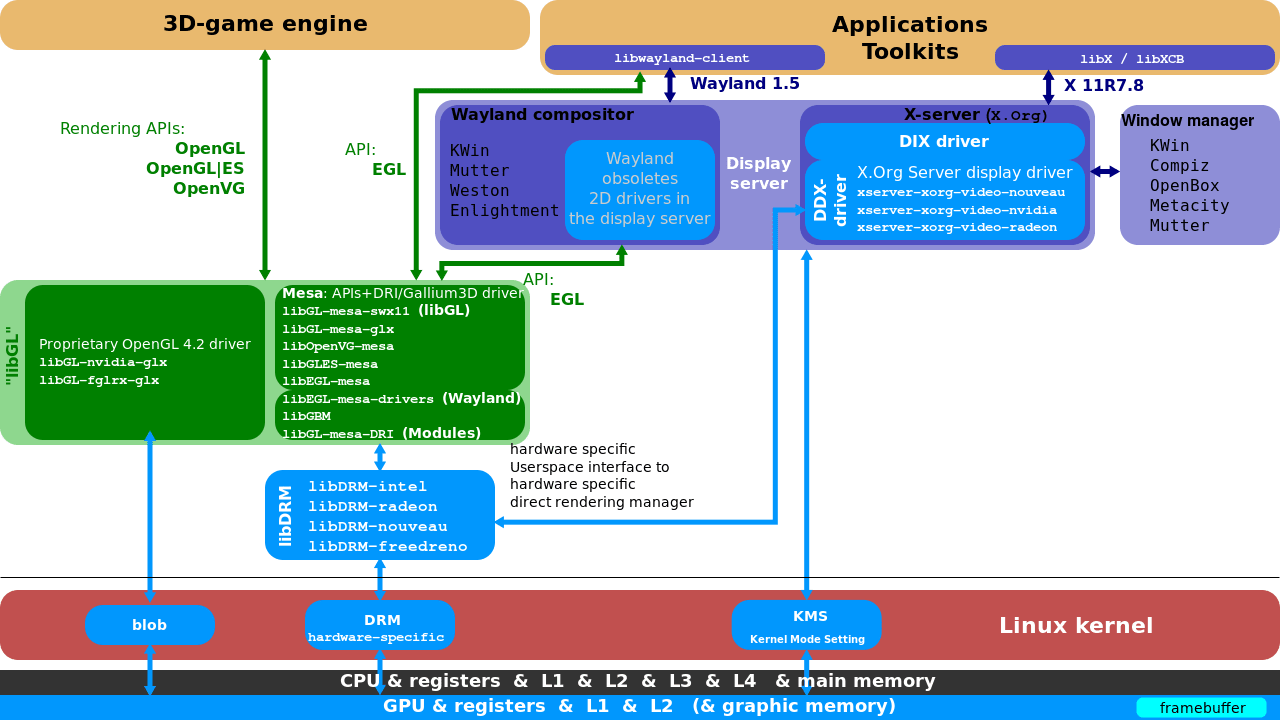
\includegraphics[width=0.75\linewidth]{linux_graphics_stack.png}}
    \caption{Illustration of the Linux graphics stack.}
    \label{img:linux_graphics_stack}
\end{figure} 

Another key component is Mesa, a free and open-source implementation of the
OpenGL specification allowing
programs to output accelerated 3D graphics inside the Linux environment. Fortunately,
DRI is conceived to run without the brokering of the X server, but it is still
needed to allocate to Mesa a surface on the display to output to. Moreover, from
an high-level perspective the communication between Mesa and the GPU works by
exchanginc commands (eg. ``draw a point'') and data (eg. ``the coordinates of the
point and its color'') that are copied to a buffer shared with the graphics hardware.


\section{WebGL} \label{sec:webgl}
WebGL is a Javascript standard API for rendering 3D graphics within any compatible
desktop or mobile web browser\footnote{A compatibility table for all the most
common browsers can be found at the following link: \url{http://caniuse.com/#feat=webgl}.}
without any external program or toolkit. WebGL programs are composed of two parts
of code: some Javascript code, that can be mixed with any other part of a standard
HTML page which is executed by the browser, and some shader code, which is written 
in the OpenGL Shading Language (GLSL) and it is executed directly by the GPU.
WebGL APIs and are exposed to the Javascript engine of the browser through the
HTML5 canvas element. Moreover, this technology is based on the OpenGL for Embedded
Systems (ES),
which is a subset of standard OpenGL library and it is both
royalty-free and open-source\footnote{The WebGL source code can be found on GitHub
at the following link: \url{https://github.com/KhronosGroup/WebGL}.}.

In the last few years a lot of frameworks and utility libraries have been developed
and the huge capabilities of these 3D graphics APIs become visible to everybody.
A lot of libraries have been built upon WebGL to render scenes and 3D objects, such
as BabylonJS~\cite{babylon3d}, three.js~\cite{cabello2010three}, and 
Cesium~\cite{cozzi20113d} (see Section \ref{sec:cesium} for a more detailed description).
Moreover, there also has been a rapid emergence~\cite{parisi2014programming} of
game engines exploiting this technology like the Unreal Engine~\cite{games2007unreal}
and Unity~\cite{engine9unity}.

The reason why the 3D navigator developed in this work uses a framework built on
WebGL is that it is, at the time of writing, the only open-source alternative to
build 3D maps inside a browser. This choiche allows to write Javascript source
code to develop the application and, at the same time, to exploit the power of
a GPU using a framweork that takes care of implementing the shaders programs.
To be more precise, looking at the whole system architecture shown in Figure
\ref{img:system_arch}, WebGL is a technology that lie inside the browser
(in this specific case Google Chrome and its Skia\footnote{\url{https://skia.org}.}
graphics engine). The browser is the one responsible for communicating with
the actual implementation of OpenGL, which is Mesa in this case study.


\section{Cesium framework} \label{sec:cesium}
Cesium\footnote{\url{https://github.com/AnalyticalGraphicsInc/cesium}.} is an
open-source JavaScript library for building 3D globes and maps.
It is one of the leading technologies in the
field and its main characteristic is to achieve the ``best possible performance,
precision, visual quality, platform support, community, and ease of use''.
As previously described in Section \ref{sec:webgl}, it is one among a wide
possibility of frameworks for building interactive 3D maps. Cesium is chosen to
build the core of the navigator application for its outstanding performances,
its well written documentation and because it is also very easy to use. This last aspect
may not seem so important at a first glance; on the other hand, when dealing with
complex systems like the FriWalk it is very important to wisely choose all its building
blocks so that they can be successfully integrated to build the system as a whole
final product. Moreover, Cesium is actively developed and maintained by a company
whose main interest is delivering the best possible library for powering its
map-based software.

\subsection{Cesium's Renderer architechture}
One of the most important features of the Cesium framework is its custom WebGL engine
called \emph{Renderer}.
It is built on the author's previous experience developing
other 3D globes libraries, which is explained in very detail in~\cite{cozzi20113d},
and it is responsible for collecting every interaction with WebGL in a single place.

Instead of scattering WebGL function calls all over the library, the centralization
of the Renderer has many and important benefits. First of all, it makes the
library very easy to use from the developer point of view, since it acts as an
intermediate layer of abstraction with respect to the plain WebGL calls. Furthermore,
it allows Cesium to build its runtime shader pipeline and its GLSL library. Last
but not least, optimizing the Renderer code through caching techniques allows
to highly improve performances allowing every other part of the framework to
benefit from it. As it is possible to see from Figure \ref{img:cesium_renderer},
the Renderer is composed of the following main parts:
\begin{itemize}
    \item the \emph{VertexArray} is a container of vertex attributes and indices
        which are stored in some internal buffers to reduce to the minimum the
        number of WebGL calls.
    \item the \emph{RenderState} includes all the WebGL functions states needed to
        perform a draw call. For example, it contains depth, blending and stencil
        states,
    \item the \emph{ShaderProgram} is a compiled/linked program with all its
        uniform matrix operations.
    \item the \emph{FrameBuffer} is a container for textures/rendererbuffer
        attachments which is the actual target of a draw call.
\end{itemize}

\begin{figure}[!htb]
    \center{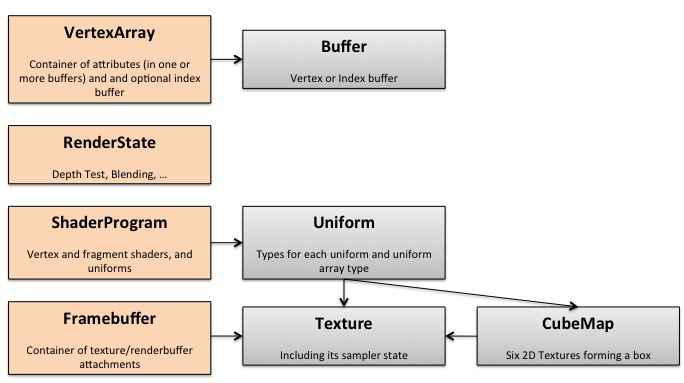
\includegraphics[width=0.55\linewidth]{cesium_renderer.jpg}}
    \caption{The components inside Cesium's Renderer.}
    \label{img:cesium_renderer}
\end{figure}

When Cesium executes a command it first binds the framebuffer (if it is different
from the previous command), then it applies the renderer states which are different
from the ones used in the last execution. Afterwards it binds\footnote{This step may
involve compiling and/or linking the shader code.} the shader program and finally it
issues a \emph{drawElements} or a \emph{drawArray} call.

Of course the Renderer is a major peculiarity of this library, but it is still only
one of its components. The Renderer uses the \emph{Scene} object to allocate and
create the WebGL resources needed for Cesium.
\begin{figure}[!htb]
    \center{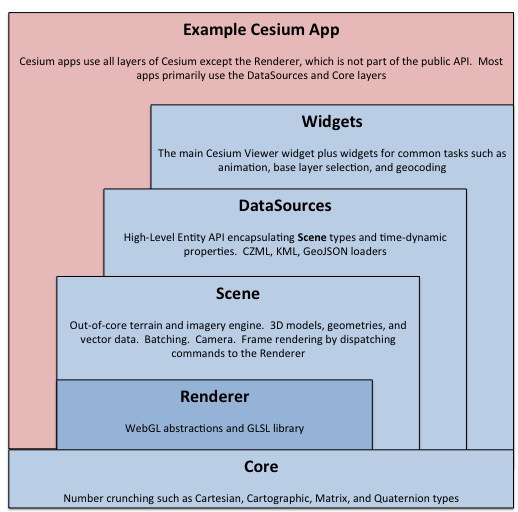
\includegraphics[width=0.45\linewidth]{cesium_stack.jpg}}
    \caption{All the components of the Cesium library.}
    \label{img:cesium_stack}
\end{figure}

Thus, as it is possible to see from Figure \ref{img:cesium_stack},
the Renderer is just a portion of the Scene component that is the ``real'' 3D
terrain and imagery engine.

Finally, as it is possible to see from Figure \ref{img:cesium_pipeline},
Cesium has a classic animate/update/render pipeline.
\begin{figure}[!htb]
    \center{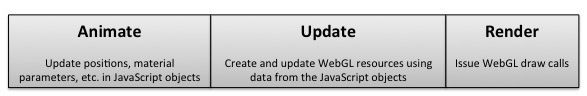
\includegraphics[width=0.6\linewidth]{cesium_pipeline.jpg}}
    \caption{The internal pipeline used in the Cesium framework.}
    \label{img:cesium_pipeline}
\end{figure}

The \emph{animate} step involves all the aspects of building each object (eg.
textures, material properties etc.) that is later rendered without interacting with
WebGL. The \emph{update} step allocates and updates all the resources needed by
WebGL using the JavaScript objects created in the previous step. Eventually, the
\emph{renderer} phase actually issues the draw calls. All the available APIs
offered by Cesium can be found in~\cite{cesiumapi}.


\section{Goole Chrome's architechture}
As previously mentioned in Section \ref{sec:friwalk_architechture}, Google Chrome
is the browser chosen for the work of this thesis. This section aims at explaining
how Google Chrome is structured internally and how it interacts with the graphics
system.

Traditionally, web browsers only relied on the CPU for all the workload produced
by the page load. Nowadays GPUs (integrated or dedicated) are a very common piece
of hardware that almost every computer and smartphone owns. Hence a lot of attention
has been payed to the ability of graphics hardware of compositing also web pages
content much faster with respect to using only the CPU. Exploiting GPUs in a web
browser not only allows to use specific hardware for drawing pixels, but also to
enhence the parallelism between CPU and GPU, which can work together for building
a very optimized rendering pipeline. To better understand how GPU comes into play
inside Google Chrome, the notion of \emph{compositor}~\cite{gpucompositing} has to
be described first.
The compositor is a piece of software inside the browser that coordinates the frame
lifecycles and it manages the internal graphics data structures. The compositor
is allowed to use the GPU to perform its drawing step. In this hardware-accelerated
architechture, compositing happens directly on the GPU via calls to the specific 3D
APIs implemented by the OS instead of communicating with the renderer process via
Inter Process Communication (IPC) and shared memory for the bitmaps representing
the page content.

Having said that, it is crucial to explain Google Chrome's renderer process issues
commands to the GPU. First of all, in the multi-process nature of the web browser
there exists a dedicated process for this task: the \emph{GPU process}. The existance
of the GPU process is a design decision made by Google's engineers mainly for
security concenrns. This is due to the sandbox protecting each renderer process
in Chrome, which means that it cannot directly issue calls to the 3D graphics APIs
made available by the OS (eg. OpenGL). For this reason it is the GPU process' job
to take care of this part of the rendering pipeline, since it is specifically
designed to provide access to the system's 3D graphics APIs from within the renderer
process sandbox.
As it is possible to see from Figure \ref{img:chrome_gpu_compositing}, Chrome's
GPU interaction happens via a client-server model.
\begin{figure}[!htb]
    \center{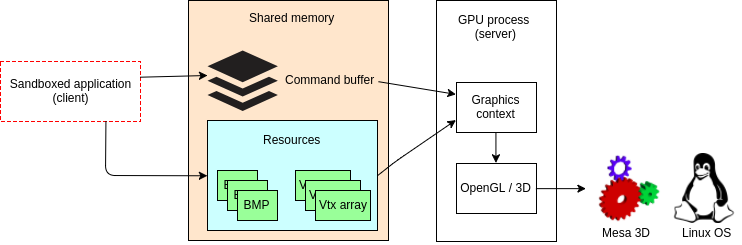
\includegraphics[width=0.8\linewidth]{chrome_gpu_architechture.png}}
    \caption{Google Chrome's GPU compositing.}
    \label{img:chrome_gpu_compositing}
\end{figure}

The flow of information works as follows:
\begin{itemize}
    \item the \emph{client} (ie. code running inside the renderer process) serializes
        calls for the system's 3D graphics into a ring buffer called
        \emph{command buffer}~\cite{gpucommandbffer}. The command buffer is a portion
        of memory which is shared between itself and the server counterpart of
        the architechture.
    \item the \emph{server} (ie. the GPU process) runs in a less restrictive sandbox
        and is allowed to access the 3D APIs available on the system. It takes the
        serialized commands which are into the buffer, it parses them and finally it
        issues the graphics calls to the Mesa driver.
\end{itemize}
